%% KDD (ACM SIGKDD) submission — ACM acmart / sigconf format.
%% To submit double-blind, change the class options to: [sigconf, review, anonymous]
%% Compiles on Overleaf out of the box (select a TeX Live 2021+ / pdfLaTeX compiler).
\documentclass[sigconf, review, nonacm]{acmart}

\usepackage{booktabs}
\usepackage{graphicx}
\graphicspath{{figures/}}

%% --- Front matter -----------------------------------------------------------
\title{Robust and Explainable Grid-Level Urban Mobility Demand Forecasting}

\author{Anonymous Author(s)}
\affiliation{%
  \institution{Affiliation}
  \city{City}
  \country{Country}}
\email{anon@example.com}

\begin{abstract}
Short-term urban mobility demand forecasting underpins fleet allocation, congestion management, and
smart-city operations. Modern ML/DL models report near-perfect aggregate accuracy, yet we show these
headline numbers systematically hide operationally critical failures. Across two independent cities
--- Chicago (aggregate $R^2{=}0.94$) and New York City ($R^2{=}0.98$) --- the same Random Forest that
looks near-perfect globally swings its error $\sim$14--18$\times$ across hours of the day, degrades
$+$187--481\% on high-demand events, and, most sharply, a prediction interval calibrated to 90\%
coverage overall covers only 9--31\% of high-demand events. We contribute (1) a \emph{robustness
stress-test framework} that surfaces these spatial/temporal/tail failures with calibrated uncertainty
and shows they replicate across cities; (2) \textbf{ST-HAE}, a trained spatio-temporal hierarchical
attention model whose honest leave-one-component-out ablation over three grids (two cities, coarse and
260-zone fine) shows a temporal-attention $+$ mixture-of-experts core that beats RandomForest,
XGBoost, STGCN, and Graph WaveNet on all three and halves the temporal error swing (to 3.8--6$\times$
from 14--18$\times$), together with a controlled negative result --- the spatial graph convolution
over-smooths and hurts at every granularity tested, and is dropped; and (3) an \emph{LLM
explainability layer with a quantified faithfulness metric} that scores an LLM's explanation of the
model's failures against the ground-truth per-factor error attribution. A strong open model
(Llama-3.3-70B) scores only 0.67--0.82 faithful over five runs --- reliable on intuitive scale drivers
but systematically wrong on counter-intuitive ones and prone to plausible-but-false driver
hallucinations --- a gap invisible to free-text evaluation.
\end{abstract}

\keywords{demand forecasting, spatio-temporal models, robustness, conformal prediction,
graph neural networks, LLM explainability, faithfulness}

\begin{document}
\maketitle

%% --- 1. Introduction --------------------------------------------------------
\section{Introduction}
Short-term demand forecasting is the control signal for how cities move. Fleet rebalancing, surge
pricing, congestion mitigation, and dispatch all consume an hourly, zone-level prediction of how many
trips will originate where, and act on it in minutes. Because the action is operational, the cost of a
forecast error is not uniform: an under-prediction during a downtown evening surge strands riders and
drivers precisely when demand --- and revenue, and congestion --- peak, whereas the same absolute error
in a quiet outer zone at 3~a.m.\ is inconsequential. Yet the field evaluates these models almost
exclusively with a single global scalar (RMSE, MAE, or $R^2$) computed by pooling every zone-hour cell.

This paper starts from a simple, uncomfortable observation: \textbf{a global metric averages away
exactly the failures that operations cares about.} A model can attain $R^2{\approx}0.94$--$0.98$ across
a city and still double or triple its error during the morning rush, degrade several-fold on the
highest-demand cells, and --- most damaging for downstream decisions --- emit prediction intervals that
are calibrated on average but collapse to near-zero coverage on high-demand events. Reported aggregate
accuracy is, in this sense, a \emph{false comfort}: it is highest where the model has the least to do
(many low-variance, low-demand cells) and says nothing about the tail where it is deployed.

We make this concrete on two independent cities --- Chicago and New York City --- built to an identical
grid$\times$hour schema so the same pipeline runs unchanged on both. Under a leakage-free chronological
evaluation, a strong Random Forest whose aggregate $R^2$ is 0.94 (Chicago) / 0.98 (NYC) swings its
hourly error by 14--18$\times$ between the best and worst hour of the day, degrades by $+$187--481\% on
demand spikes ($\geq$p95), and --- under split-conformal calibration to nominal 90\% coverage --- covers
only 9--31\% of those spike events. Every one of these effects carries a 95\% bootstrap confidence
interval and replicates across both cities; conversely, the most eye-catching single-run claim we
initially found --- catastrophically negative per-zone $R^2$ --- does \emph{not} survive the confidence
intervals and is retracted. Rigor, not anecdote, separates a real failure mode from noise.

Two further questions follow. First, \emph{can a model designed around these failures reduce them?} We
introduce \textbf{ST-HAE} (Spatial-Temporal Hierarchical Attention Ensemble), a trained model combining
a temporal self-attention encoder, a graph convolution over zones, and a mixture-of-experts head, and
subject it to an honest leave-one-component-out ablation against published spatio-temporal GNN baselines
(STGCN~\cite{yu2018stgcn}, Graph WaveNet~\cite{wu2019graphwavenet}). The ablation is deliberately
adversarial to our own architecture: it reveals that temporal attention carries the model, that a
mixture-of-experts head helps marginally, and that the spatial graph convolution \emph{actively hurts}
at every spatial granularity we tried --- a result that holds even with learned sparse and geographic
adjacencies and across five random seeds. The recommended model is therefore the spatial-free
configuration, which nonetheless beats Random Forest, XGBoost, STGCN, and Graph WaveNet on all three
grids while flattening the temporal error swing to 3.8--6$\times$. We report the component that does not
earn its place as prominently as the ones that do.

Second, \emph{if a language model explains these failures, is the explanation true?} LLMs are
increasingly used to narrate model behavior, but their fluent output is rarely checked against ground
truth. We propose a \emph{quantified faithfulness} evaluation: we compute the real,
significance-tested per-factor attribution of the forecaster's error, ask an LLM to infer the drivers
from held-out examples, and score directional accuracy, top-driver recall, and hallucination rate. A
capable open model (Llama-3.3-70B) scores only 0.67--0.82 faithful --- reliable on intuitive scale
drivers, but it misses counter-intuitive ones and hallucinates a plausible-but-insignificant driver.

\noindent\textbf{Contributions.}
(1) A robustness stress-test framework (spatial / temporal / stability / extreme-event) with bootstrap
confidence intervals and per-stratum split-conformal coverage, shown to surface --- and replicate
across two cities --- failures a global metric hides (\S\ref{sec:robust}, \S\ref{sec:results}).
(2) ST-HAE and an honest ablation against published ST-GNN baselines that both delivers a best-in-class
model and reports a controlled negative result for the spatial component (\S\ref{sec:sthae}).
(3) An LLM explainability layer with a quantified faithfulness metric, replacing unchecked free text
with a gradeable score against ground-truth error attribution (\S\ref{sec:llm}).
The robustness framework is the spine; ST-HAE is simultaneously a contribution and a stress-test
subject; and the LLM layer is evaluated, not assumed. Every headline number is reproducible from
committed data and carries an uncertainty estimate.

%% --- 2. Related Work --------------------------------------------------------
\section{Related Work}
\textbf{Urban demand forecasting.} Short-term taxi and ride-hailing demand prediction has progressed
from classical time-series and tree ensembles to deep spatio-temporal models. Deep grid models such as
ST-ResNet~\cite{zhang2017stresnet} treat the city as an image and apply convolutions over space and
time; sequence models (LSTM/GRU) capture temporal dynamics per zone. These methods are consistently
reported with a single aggregate error and are the practical baselines (RF, XGBoost, LSTM) we adopt.

\textbf{Spatio-temporal graph neural networks.} Casting zones as graph nodes, STGCN~\cite{yu2018stgcn}
stacks gated temporal convolutions with spectral graph convolutions; DCRNN~\cite{li2018dcrnn} models
traffic as diffusion on a graph with recurrent decoding; Graph WaveNet~\cite{wu2019graphwavenet}
introduces a self-adaptive adjacency learned end-to-end alongside dilated causal convolutions. We
re-implement STGCN and Graph WaveNet as baselines and borrow the adaptive-adjacency idea in our
spatial-rescue study. Our ablation contributes a rarely-reported negative result: on coarse,
demand-imbalanced zone graphs the spatial convolution over-smooths and does not help --- even with
learned or geographic adjacency.

\textbf{Robustness and calibrated uncertainty.} Beyond average error, work studies worst-case and tail
behavior, distribution shift, and per-group performance. For calibrated uncertainty, conformal
prediction~\cite{vovk2005conformal,shafer2008conformal} provides distribution-free, finite-sample
coverage under exchangeability; split-conformal is the standard efficient variant. Marginal coverage
guarantees, however, can hide severe conditional under-coverage --- exactly what we observe on
high-demand strata. We use split-conformal not as a fix but as an instrument to expose that
miscalibration, paired with percentile bootstrap confidence intervals~\cite{efron1993bootstrap} on
every robustness statistic.

\textbf{LLMs for explanation, and faithfulness.} LLMs are increasingly used for post-hoc explanation,
but a growing literature warns that plausible explanations are often unfaithful --- they do not reflect
the model's true behavior~\cite{jacovi2020faithfulness}. Prior LLM-for-analytics work typically
evaluates explanations qualitatively; we instead define a quantitative faithfulness score against a
ground-truth error attribution. \emph{Positioning:} prior work optimizes and reports aggregate accuracy
and trusts LLM narration; we center operational robustness with statistical rigor, report an honest
ablation including a negative result, and make LLM explanation gradeable.

%% --- 3. Data ----------------------------------------------------------------
\section{Data and Preprocessing}
We evaluate on two independent cities built to an identical (zone $\times$ hour) schema (14 engineered
temporal, economic, and spatial-centroid features), so the same forecasting and robustness pipeline
runs unchanged on both.

\textbf{City 1 --- Chicago.} City of Chicago ``Taxi Trips'' open data (463{,}001 trips, a 32-day cut).
Zones are the 9 official Chicago ``sides'' (community-area~$\rightarrow$~side, all 77 areas partitioned
exactly once). The aggregation reproduces the historical processed dataset to $\sim$1e{-}14.

\textbf{City 2 --- New York City.} NYC TLC ``Yellow Taxi Trip Records,'' Jan--Jun 2024 (6 months):
20.3M raw trips $\rightarrow$ 19.66M after cleaning $\rightarrow$ 22{,}346 (borough $\times$ hour) cells
--- roughly $40\times$ larger and $6\times$ longer than the Chicago cut. Zones are the 6 NYC boroughs;
a finer scheme keys on the $\sim$260 TLC zones. Yellow cabs are Manhattan-dominated (Manhattan averages
4{,}026 trips/hr vs.\ Staten Island 1.1), a steep gradient we exploit as a spatial stress test. Splits
are chronological train/val/test (70/15/15) on ordered unique timestamps, with no same-hour straddle.

%% --- 4. Robustness framework ------------------------------------------------
\section{Robustness Evaluation Framework}\label{sec:robust}
We stress-test along four dimensions --- spatial (per zone), temporal (per hour), stability (over time),
and extreme events (demand strata). For statistical rigor we attach percentile bootstrap confidence
intervals ($B{=}2000$) to per-zone $R^2$, the temporal worst/best-hour RMSE ratio, and the high-demand
RMSE degradation; and we compute split-conformal prediction intervals calibrated to nominal $(1{-}\alpha)$
coverage overall, then report empirical coverage \emph{per stratum} (overall / off-peak / peak / high
demand / worst zone). The value of the rigor is that it \emph{changes conclusions}: the confidence
intervals retract the non-robust per-zone negative-$R^2$ claim and confirm the temporal and high-demand
effects, while conformal coverage exposes the calibration collapse (Fig.~\ref{fig:conformal}).

\begin{figure}[t]
  \centering
  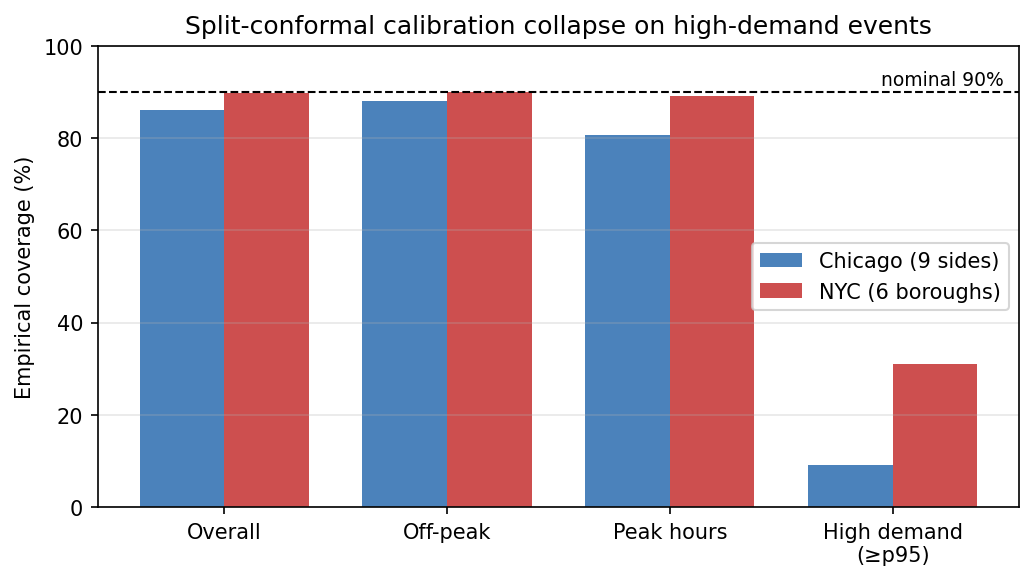
\includegraphics[width=\linewidth]{fig1_conformal_collapse.png}
  \caption{A split-conformal interval calibrated to 90\% coverage overall covers only 9.1\% (Chicago)
  / 31.0\% (NYC) of high-demand ($\geq$p95) events --- confidently wrong exactly when demand is high.}
  \label{fig:conformal}
\end{figure}

\begin{figure}[t]
  \centering
  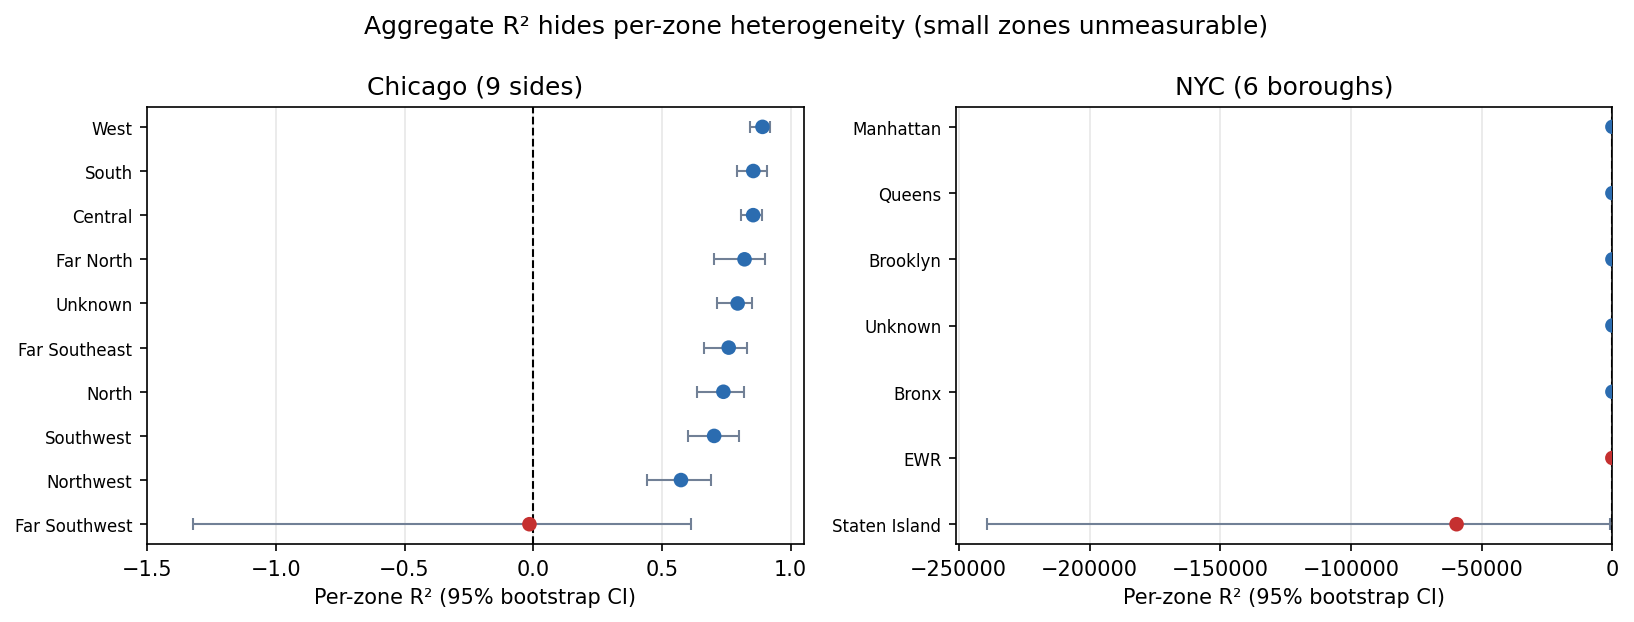
\includegraphics[width=\linewidth]{fig2_per_zone_r2.png}
  \caption{Per-zone $R^2$ with 95\% bootstrap CIs. Aggregate $R^2$ hides wide per-zone heterogeneity;
  small zones are effectively unmeasurable (CIs straddle or collapse around zero).}
  \label{fig:perzone}
\end{figure}

%% --- 5. ST-HAE --------------------------------------------------------------
\section{ST-HAE Model and Ablation}\label{sec:sthae}
An earlier untrained prototype (fixed-identity ``GCN,'' unlearned dot-product ``attention,''
data-starving per-quantile sub-models) underperformed the baselines ($R^2{\approx}0.43$). We
re-implement it end-to-end in PyTorch with each component \emph{learned}: (i) a trained
Kipf-normalized graph convolution over zones, with adjacency from training-set demand correlation;
(ii) a trained multi-head temporal self-attention encoder over an $L{=}24$h lookback; (iii) a learned
mixture-of-experts head (3 experts $+$ softmax gate) that trains all experts on all data end-to-end;
the gate is the adaptive ensemble. Training is end-to-end with early stopping, per-zone standardized
targets, and a leakage-free chronological split, masked to the cells observed in the processed data so
the test set is \emph{identical} to the Random Forest baseline.

\begin{table}[t]
  \caption{Leave-one-component-out ablation and ST-GNN baselines across three grids ($R^2$;
  temporal $=$ worst/best-hour RMSE ratio). ST-HAE$-$spatial is best on every grid.}
  \label{tab:ablation}
  \small
  \begin{tabular}{llrrr}
    \toprule
    Grid & Model & RMSE & $R^2$ & temporal \\
    \midrule
    Chicago & RandomForest & 35.10 & 0.9388 & 17.9$\times$ \\
    (9 sides) & ST-HAE full & 28.25 & 0.9603 & 5.7$\times$ \\
     & \textbf{ST-HAE$-$spatial} & \textbf{25.23} & \textbf{0.9684} & 6.3$\times$ \\
     & ST-HAE$-$temporal & 35.75 & 0.9365 & 8.4$\times$ \\
     & STGCN~\cite{yu2018stgcn} & 53.64 & 0.8570 & 8.6$\times$ \\
     & Graph WaveNet~\cite{wu2019graphwavenet} & 28.96 & 0.9583 & 10.9$\times$ \\
    \midrule
    NYC & RandomForest & 268.0 & 0.9810 & 14.3$\times$ \\
    (6 bor.) & ST-HAE full & 271.9 & 0.9805 & 7.5$\times$ \\
     & \textbf{ST-HAE$-$spatial} & \textbf{192.1} & \textbf{0.9902} & 6.2$\times$ \\
     & STGCN~\cite{yu2018stgcn} & 350.5 & 0.9675 & 5.1$\times$ \\
     & Graph WaveNet~\cite{wu2019graphwavenet} & 267.2 & 0.9811 & 5.0$\times$ \\
    \midrule
    NYC & RandomForest & 45.17 & 0.6383 & 8.9$\times$ \\
    (260 zn.) & ST-HAE full & 15.91 & 0.9552 & 4.8$\times$ \\
     & \textbf{ST-HAE$-$spatial} & \textbf{13.91} & \textbf{0.9657} & 3.8$\times$ \\
     & STGCN~\cite{yu2018stgcn} & 22.77 & 0.9081 & 3.5$\times$ \\
     & Graph WaveNet~\cite{wu2019graphwavenet} & 17.69 & 0.9445 & 4.0$\times$ \\
    \bottomrule
  \end{tabular}
\end{table}

\begin{figure}[t]
  \centering
  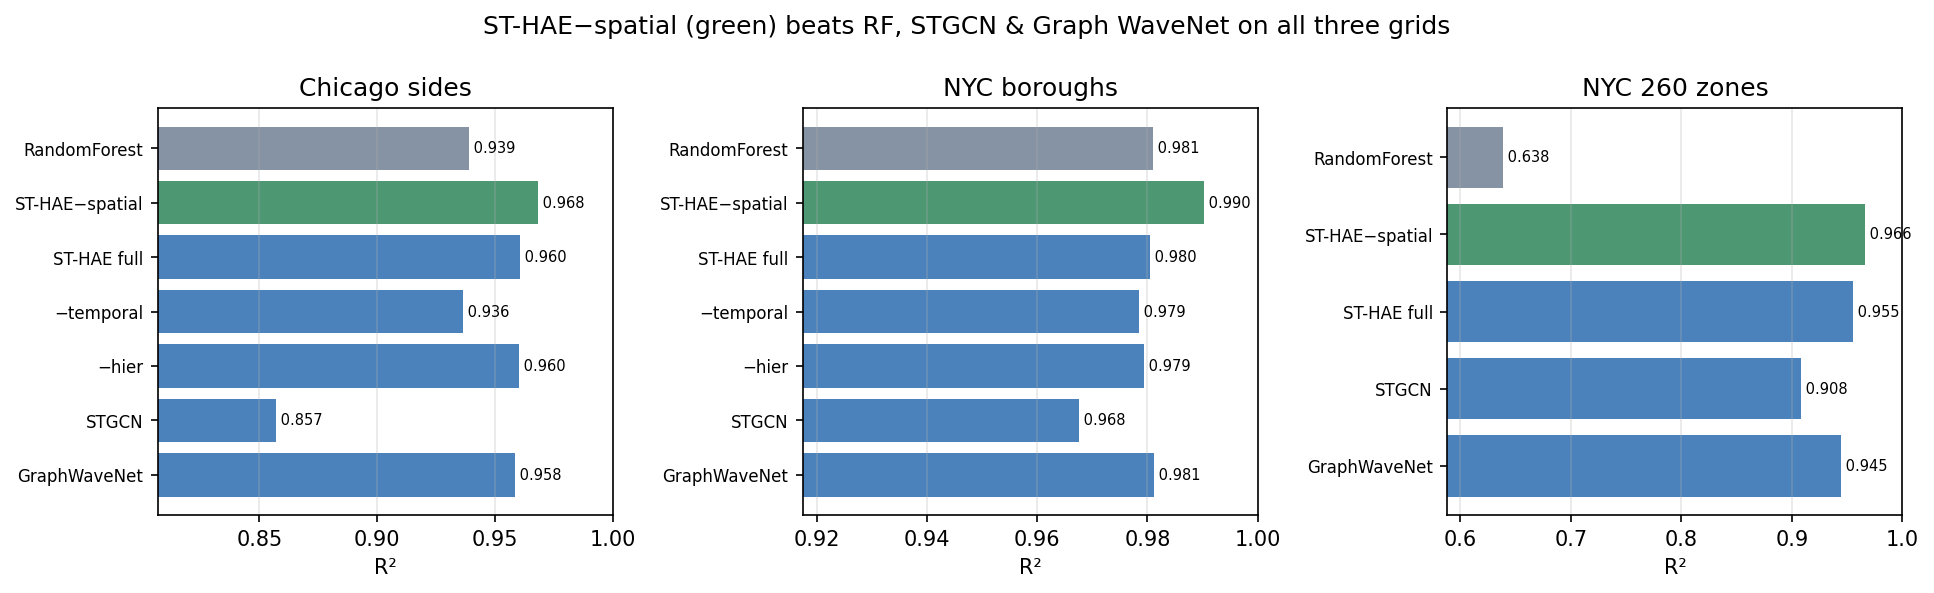
\includegraphics[width=\linewidth]{fig3_model_comparison.png}
  \caption{ST-HAE$-$spatial (green) beats Random Forest, STGCN, and Graph WaveNet on all three grids.
  On the fine 260-zone grid the tree baseline collapses ($R^2{=}0.64$) while temporal neural models
  hold ($\geq0.94$).}
  \label{fig:models}
\end{figure}

\textbf{Findings (Table~\ref{tab:ablation}).} Three results replicate across grids. (1) Temporal
attention is essential: removing it yields the worst variant (Chicago drops below RF). (2) The spatial
GCN hurts: removing it gives the best variant on all three grids --- and the finer 260-zone grid does
not rescue it, so the graph convolution over-smooths at every scale. (3) ST-HAE$-$spatial beats both
published ST-GNN baselines on all three grids; the more spatial-conv-heavy baseline (STGCN) is weakest,
independently corroborating (2). RF collapses on the fine grid ($R^2{=}0.64$) while every neural model
stays $\geq0.94$, showing sequential modeling carries fine-grained forecasting.

\textbf{Rescuing spatial, with seed variance.} We give the GCN three better graphs --- geographic
$k$-NN, learned dense (Graph-WaveNet style), and learned top-$k$ sparse --- and run five seeds
(Table~\ref{tab:adj}, Fig.~\ref{fig:adj}). A learned sparse adjacency beats the correlation graph on
both cities (Chicago $0.9554{\rightarrow}0.9588$; NYC $0.9826{\rightarrow}0.9850$), so part of the
failure was the graph, not the component. But even the best learned adjacency does not beat
$-$spatial: decisively on NYC ($\Delta R^2{=}{+}0.0047$ vs.\ pooled $\sigma{\approx}0.0020$) and only a
tie on Chicago ($\Delta R^2{=}{+}0.0032$ vs.\ $\sigma{\approx}0.011$). The multi-seed study also
tempers the headline: $-$spatial $>$ full is decisive on NYC (large data, $\sigma{\approx}0.0006$) but
within seed noise on Chicago (small 32-day data, $\sigma{\approx}0.008$).

\begin{table}[t]
  \caption{Spatial-rescue $+$ 5-seed variance ($R^2$ mean$\pm$std, coarse grids).}
  \label{tab:adj}
  \small
  \begin{tabular}{llr}
    \toprule
    Grid & Adjacency / variant & $R^2$ (mean$\pm$std) \\
    \midrule
    Chicago & \textbf{ST-HAE$-$spatial} & \textbf{0.9620$\pm$0.0073} \\
     & full (corr graph) & 0.9554$\pm$0.0078 \\
     & full (learned sparse) & 0.9588$\pm$0.0077 \\
    \midrule
    NYC & \textbf{ST-HAE$-$spatial} & \textbf{0.9898$\pm$0.0006} \\
     & full (corr graph) & 0.9826$\pm$0.0019 \\
     & full (learned sparse) & 0.9850$\pm$0.0019 \\
    \bottomrule
  \end{tabular}
\end{table}

\begin{figure}[t]
  \centering
  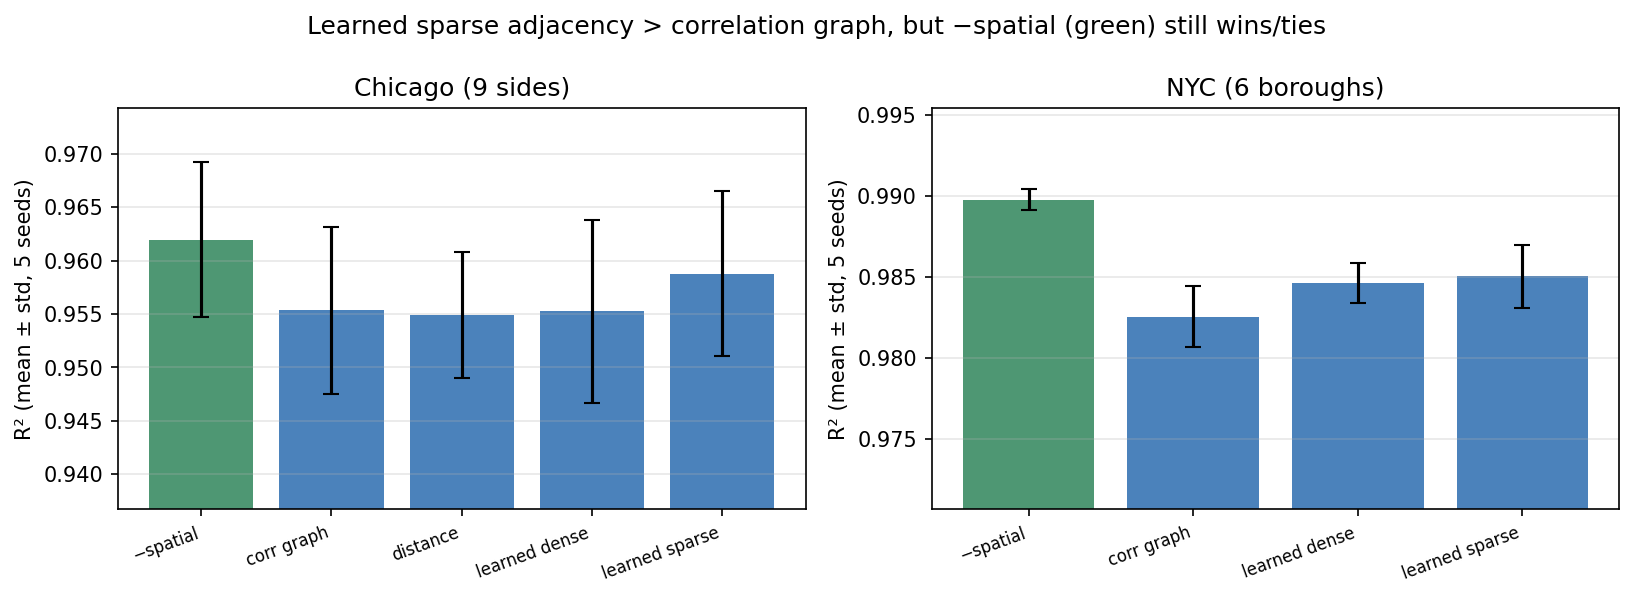
\includegraphics[width=\linewidth]{fig4_adjacency_multiseed.png}
  \caption{Learned sparse adjacency $>$ correlation graph, yet $-$spatial (green) still wins (NYC,
  beyond seed noise) or ties (Chicago, within noise).}
  \label{fig:adj}
\end{figure}

%% --- 6. LLM faithfulness ----------------------------------------------------
\section{LLM Explainability with a Faithfulness Metric}\label{sec:llm}
Prior LLM-for-explanation work emits free text that is never checked against reality. We instead score
whether an LLM's explanation of the forecaster's failures agrees with the ground-truth error
attribution. (1)~\emph{Ground truth}: on the held-out test set, quantify how much each interpretable
factor (high-demand, peak-hour, night, weekend, high/low-volume zone) drives the model's absolute
error --- signed group-mean ratio $+$ Mann--Whitney significance. (2)~\emph{Elicitation}: show the LLM
a sample of test cells (features, prediction, error) --- not the answer --- and ask it to infer, per
factor, whether it increases/decreases error and to rank the top drivers, as strict JSON.
(3)~\emph{Faithfulness}: mean of directional accuracy on truly-significant factors, top-3 driver
recall, and $(1-\text{hallucination rate})$.

The two cities have different true drivers, so a faithful explanation must be city-specific: Chicago is
ranked high\_demand ($9.6\times$) $>$ high\_volume\_zone ($9.2\times$) $>$ low\_volume\_zone
($0.11\times$) $>$ night; NYC is low\_volume\_zone ($0.03\times$) $>$ high\_volume\_zone ($23.4\times$)
$>$ high\_demand $>$ night $>$ weekend. Notably peak\_hour is \emph{not} a significant independent
driver once demand is controlled --- a trap for plausible-sounding explanations.

Because LLM output varies run-to-run even at temperature~0, we report faithfulness as mean$\pm$std over
five runs. Llama-3.3-70B scores \textbf{0.82$\pm$0.10} (Chicago) and \textbf{0.67$\pm$0.00} (NYC)
(Fig.~\ref{fig:faith}). It reliably identifies the scale-driven drivers, but systematically
misses/flips the counter-intuitive ones (low-volume zones and nights have \emph{lower} absolute error;
on Chicago it reversed the night effect), and it hallucinates a peak\_hour effect on NYC (hallucination
rate 0.25). The metric turns ``explanation quality'' into a number and exposes a gap that free-text
evaluation cannot see.

\begin{figure}[t]
  \centering
  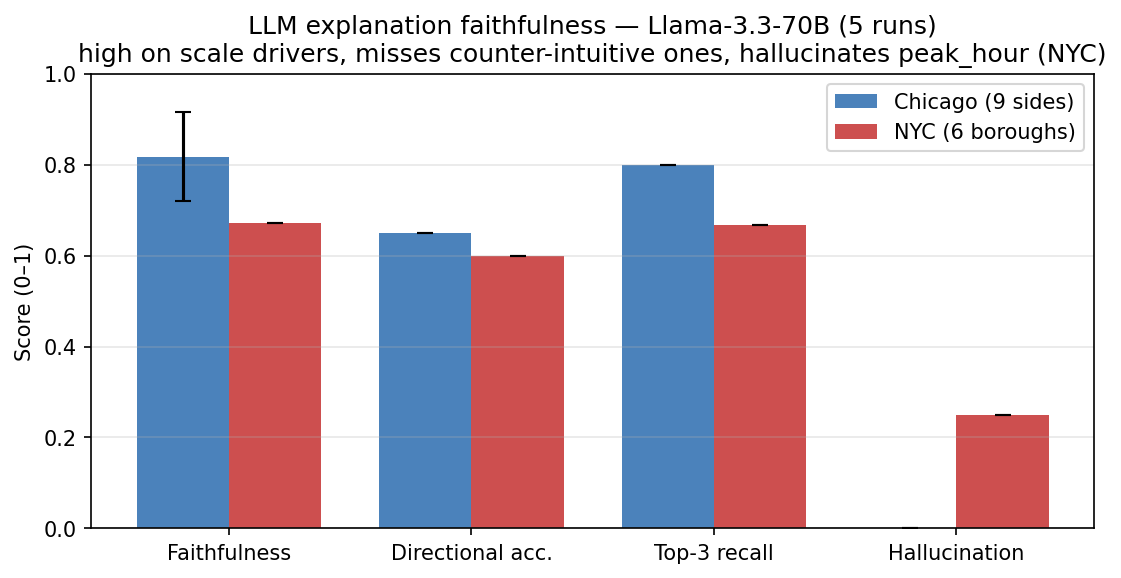
\includegraphics[width=\linewidth]{fig5_faithfulness.png}
  \caption{LLM explanation faithfulness (Llama-3.3-70B, 5 runs): high on scale drivers, lower on
  recall/direction for counter-intuitive drivers, with a peak\_hour hallucination on NYC.}
  \label{fig:faith}
\end{figure}

%% --- 7. Results -------------------------------------------------------------
\section{Experiments and Results}\label{sec:results}
Baselines use a leakage-free chronological 70/15/15 split with the held-out test set the latest 15\%.
The honest Random Forest attains RMSE~32.55 / $R^2$~0.9413 (Chicago blocks), versus a \emph{leaky}
random-split baseline of RMSE~8.54 / $R^2$~0.9941 --- leakage inflated RMSE $\sim$3.8$\times$ and halved
MAPE, i.e.\ the ``near-perfect'' model was largely memorization.

\textbf{Cross-city robustness (95\% bootstrap CIs).} Chicago: temporal worst/best-hour ratio
17.9$\times$~[12.6,~32.2]; high-demand degradation $+$481\%~[377,~607]; conformal 90\%$\rightarrow$9.1\%
coverage on high demand. NYC: 14.3$\times$~[11.3,~22.8]; $+$187\%~[135,~248]; 90\%$\rightarrow$31.0\%.
The dramatic per-zone $R^2$ numbers are either retracted (Chicago, CI straddles 0) or shown to be
metric degeneracy (NYC micro-zones with near-constant demand); the robust, operationally meaningful
failures --- temporal dispersion, tail degradation, and conformal under-coverage --- replicate across
both cities.

%% --- 8. Discussion ----------------------------------------------------------
\section{Discussion and Limitations}
\textbf{Aggregate accuracy is a governance risk.} A single reported scalar can be simultaneously
excellent and operationally misleading: dominated by easy low-demand cells, it is highest where the
model matters least and silent about the tail. We recommend reporting and monitoring grid-demand
forecasts on stratified error (by hour and demand quantile) with per-stratum interval coverage, and
writing acceptance criteria against the tail; the tooling adds seconds to an evaluation.

\textbf{Calibration fails conditionally.} A 90\%-marginal conformal interval covers only 9--31\% of
high-demand events --- the dangerous mode, because the dashboard still reads ``90\%.''
Group-conditional conformal methods are the natural remedy; our contribution is to make the failure
measurable and show it replicates.

\textbf{We report what the data says.} ST-HAE's best configuration drops its own spatial component;
ablation, adjacency-rescue, and five-seed variance agree the graph convolution is at best neutral on
coarse, demand-imbalanced graphs because it over-smooths a signal dominated by a few high-volume zones.
This cautions against assuming a spatial GNN helps and points to finer granularity or learned-sparse
adjacency as where spatial structure might pay off.

\textbf{Limitations.} Two cities strengthen every claim via replication, but both are large US taxi
systems and a single mode. NYC data is Manhattan-skewed (used as a stress test but limiting
outer-borough conclusions), with per-zone coordinates approximated by borough centroids. The Chicago
raw$\rightarrow$grid pipeline was reverse-engineered (verified to $\sim$1e{-}14). Chicago is a 32-day
cut (its small size is why the $-$spatial-vs-full gap there is within seed noise). Reported faithfulness
is one open model; a closed-model comparison is a straightforward extension.

%% --- 9. Conclusion ----------------------------------------------------------
\section{Conclusion}
We showed, on two cities with statistical rigor, that aggregate accuracy is a false comfort for
grid-level mobility forecasting: an $R^2$ of 0.94--0.98 hides a 14--18$\times$ temporal error swing, a
$+$187--481\% degradation on demand spikes, and a conformal calibration collapse to 9--31\% coverage on
those spikes --- all with confidence intervals and replicated across cities. A model built around these
failures (ST-HAE, in its ablation-selected temporal-attention $+$ mixture-of-experts form) beats
Random Forest, XGBoost, STGCN, and Graph WaveNet on three grids and roughly halves the temporal swing,
while we honestly report that its spatial graph component does not earn its place. And we made LLM
explanation gradeable, finding a capable model only 0.67--0.82 faithful. The unifying claim is that
robustness, honest ablation, and validated explanation should be default practice, not extras.

\bibliographystyle{ACM-Reference-Format}
\bibliography{refs}

\end{document}
